\chapter{System Description}\label{ch:system-description}

% TODO Write some chapter introduction

% ===============
% MODEL ARCHITECTURE
% ===============

\section{Model Architecture}
 
\begin{figure}[h]
\centering
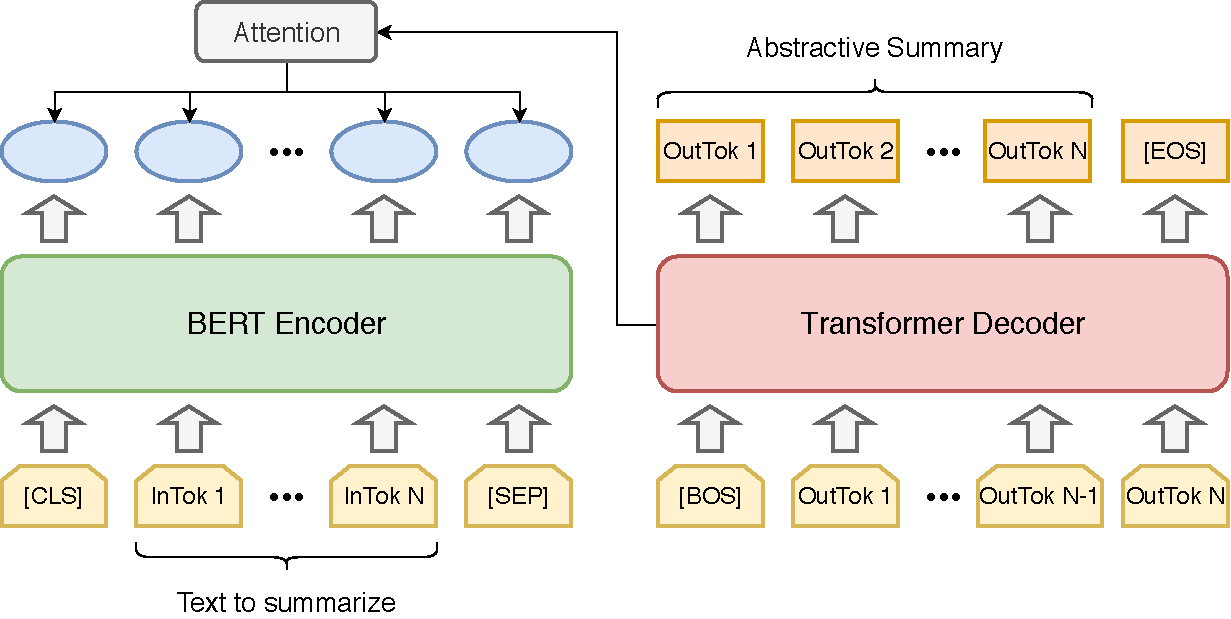
\includegraphics[width=0.7\paperwidth]{figures/summarization-architecture}
\caption{Visualization of the model architecture.}
\label{fig:summarization-architecture}
\end{figure}

The architecture of the model used in this work is pretty simple.
For the encoding part, BERT is used and for decoding, a normal Transformer decoder is used.
Like proposed in \cite{1608.05859}, the input embeddings are tied to the output layer.

As described in \cref{sec:bert}, BERT allows either one or two sentence\footnote{Remember, that sentence is not referring to an actual linguistic sentence} inputs.
For this work, only one sentence is used, as there is no need (and logical way) to split the input into two parts.
The Transformer decoder performs attentions over the full output representations of the encoder.
The full architecture is shown in \cref{fig:summarization-architecture}.

% =======
% TRAINING
% =======

\section{Training}\label{sec:system-description-training}

% TODO I'm pretty sure that there are better examples, but for now this is fine
\begin{figure}[h]
\begin{lstlisting}[numbers=none]
DA1: Thank you very much indeed,
DA2: Cool, thank you,
DA3: So I call the meeting closed.

SUM: They close the meeting by thanking one another.
\end{lstlisting}
\caption{Three dialogue acts (DA1-3) that are linked to one sentence of the summary (SUM).}
\label{fig:dialogue-arc-summary-link-example}
\end{figure}

To circumvent the high memory usage of BERT at long sequence lengths, not the whole meeting transcript is used as input for the network at once.
As described in \cref{sec:ami-meeting-corpus}, for every sentence in a meeting's abstractive summary, there exists a link to one or more dialogue acts.
These are the dialogue act, that influence the content of the sentence the most.
An example for such a link is shown in \cref{fig:dialogue-arc-summary-link-example}.
For training, all of these dialogue acts, that belong to the same summary sentence, are concatenated and used as the source for the summary.
The summary sentence itself is used as the target summary.

\subsection{Preparation of Training Data}



\subsubsection{NXT}

\subsubsection{Data Cleaning}

\subsubsection{Data Split}

% ===================
% IMPLEMENTATION WITH TEXAR
% ===================

\section{Implementation with Texar}

% ====================
% EXPLORING HYPERPARAMETERS
% ====================

\section{Exploring Hyperparemeters}